\subsection{IASI Band 2 (1210-2000\invcm)}
%-----------------------------------------

\subsubsection{WVO-derived profiles}
%...................................
Both the WVO1 and WVO2 results are similar with the most visible difference in the spectral region 1700-1850\invcm{} where the WVO1 residuals are a tiny bit noisier. The frequency of the largest maximum $\Delta T_{B}$ residual is 1363.25\invcm. Examples of the behaviour of the transmittance profiles for this channel for UMBC profile 1 (tropical) and profile 41 (polar) are shown in figures \ref{fig:iasiB2.wvo_tauprofile_p1_f1363.25} and \ref{fig:iasiB2.wvo_tauprofile_p41_f1363.25} respectively.
\begin{figure}[htp]
  \centering
  \includegraphics[scale=0.8]{graphics/iasiB2/iasiB2.wvo_tauprofile_p1_f1363.25.eps}
  \caption{IASI band 2 WVO-derived transmittance profiles for UMBC dependent set profile 1 (tropical), $f$=1363.25\invcm{} (frequency of the largest $\Delta T_{B}$ residual in figure \ref{fig:iasiB2.wvo1_dtb} and \ref{fig:iasiB2.wvo2_dtb}). The strong water vapour absorption shown in panel (a) means that numerical errors dominate the lower level effective dry and ozone transmittances shown in panels (c) and (e) respectively.}
  \label{fig:iasiB2.wvo_tauprofile_p1_f1363.25}
\end{figure}
\begin{figure}[htp]
  \centering
  \includegraphics[scale=0.8]{graphics/iasiB2/iasiB2.wvo_tauprofile_p41_f1363.25.eps}
  \caption{IASI band 2 WVO-derived transmittance profiles for UMBC dependent set profile 41 (polar), $f$=1363.25\invcm{} (frequency of the largest $\Delta T_{B}$ residual in figure \ref{fig:iasiB2.wvo1_dtb} and \ref{fig:iasiB2.wvo2_dtb}). Panel (c) shows the ``turnaround'' in the effective dry transmittance profile (and its ``correction'') that is used in both the WVO1 and WVO2 set.}
  \label{fig:iasiB2.wvo_tauprofile_p41_f1363.25}
\end{figure}


\subsubsection{DOZ-derived profiles}
%...................................
As with the WVO results, both the DOZ1 and DOZ2 results are similar. However, the magnitude of the statistics for these transmittances are nearly two orders of magnitude \emph{less} than for the WVO results across the entire band. Examination of the 1363.25\invcm{} channel transmittances for profile 1, shown in figure \ref{fig:iasiB2.doz_tauprofile_p1_f1363.25}, indicates why; comparison to the same for the WVO transmittances (see figure \ref{fig:iasiB2.wvo_tauprofile_p1_f1363.25}) shows the dominant absorbers (wet and dry) in the DOZ transmittances are much better behaved, in particular the dry transmittances. The ozone transmittances still exhibit anomalous behaviour but the contribution from ozone is almost negligible.

An interesting point to note is that the maximum difference between the LBL and DOZ-derived effective wet transmittances shown in figure \ref{fig:iasiB2.doz_tauprofile_p1_f1363.25} is an order of magnitude larger than those for the WVO-derived set, and occurs near the peak water vapour absorption whereas the peak difference for the WVO-derived effective wet transmittances occurs much lower down in the atmosphere at which point the water vapour absorption is mostly saturated so any differences would not be thought to have a large impact.
\begin{figure}[htp]
  \centering
  \includegraphics[scale=0.8]{graphics/iasiB2/iasiB2.doz_tauprofile_p1_f1363.25.eps}
  \caption{IASI band 2 DOZ-derived transmittance profiles for UMBC dependent set profile 1 (tropical), $f$=1363.25\invcm{} (frequency of the largest $\Delta T_{B}$ residual for the WVO transmittances in figure \ref{fig:iasiB2.wvo1_dtb} and \ref{fig:iasiB2.wvo2_dtb}). Compare with the WVO transmittances of figure \ref{fig:iasiB2.wvo_tauprofile_p1_f1363.25}}
  \label{fig:iasiB2.doz_tauprofile_p1_f1363.25}
\end{figure}


\subsubsection{WVD-derived profiles}
%...................................
